\tableofcontents

\newpage

\section{Решение нелинейных уравнений}

\subsection{Метод хорд}

\subsubsection{Описание метода}
\underline{Суть метода:} функция \textit{y = f(x)} на отрезке \textit{[a,b]} заменяется хордой и в качестве приближенного
значения корня принимается точка пересечения хорды с осью абсцисс.


\underline{Алгоритм метода:}
\begin{enumerate}
    \item Найти $a$ и $b$ такие, что $a*b$<$0$
    \item Вычислить $x_0$:  $x_0$=$a_0$ - $\frac{b_0-a_0}{f(b_0)-f(a_0)}$$f(a_0)$
    \item Вычислить $f(x_0)$
    \item По критерию из п.1 выбрать новый интервал: $[a_0,x_0]$ или $[x_0,b_0]$
    \item Вычислить $x_1$ и т.д., пока $|x_i - x_{i-1}|>\epsilon$; $x_i$=$\frac{a_{i}f(b_i)-b_{i}f(a_i)}{f(b_i)-f(a_i)}$
    \item Получим приближённое значение корня $x^*$=$x_n$
\end{enumerate}

\subsubsection{Блок-схема численного метода}
b%\begin{figure}[H]
%    \centering
%    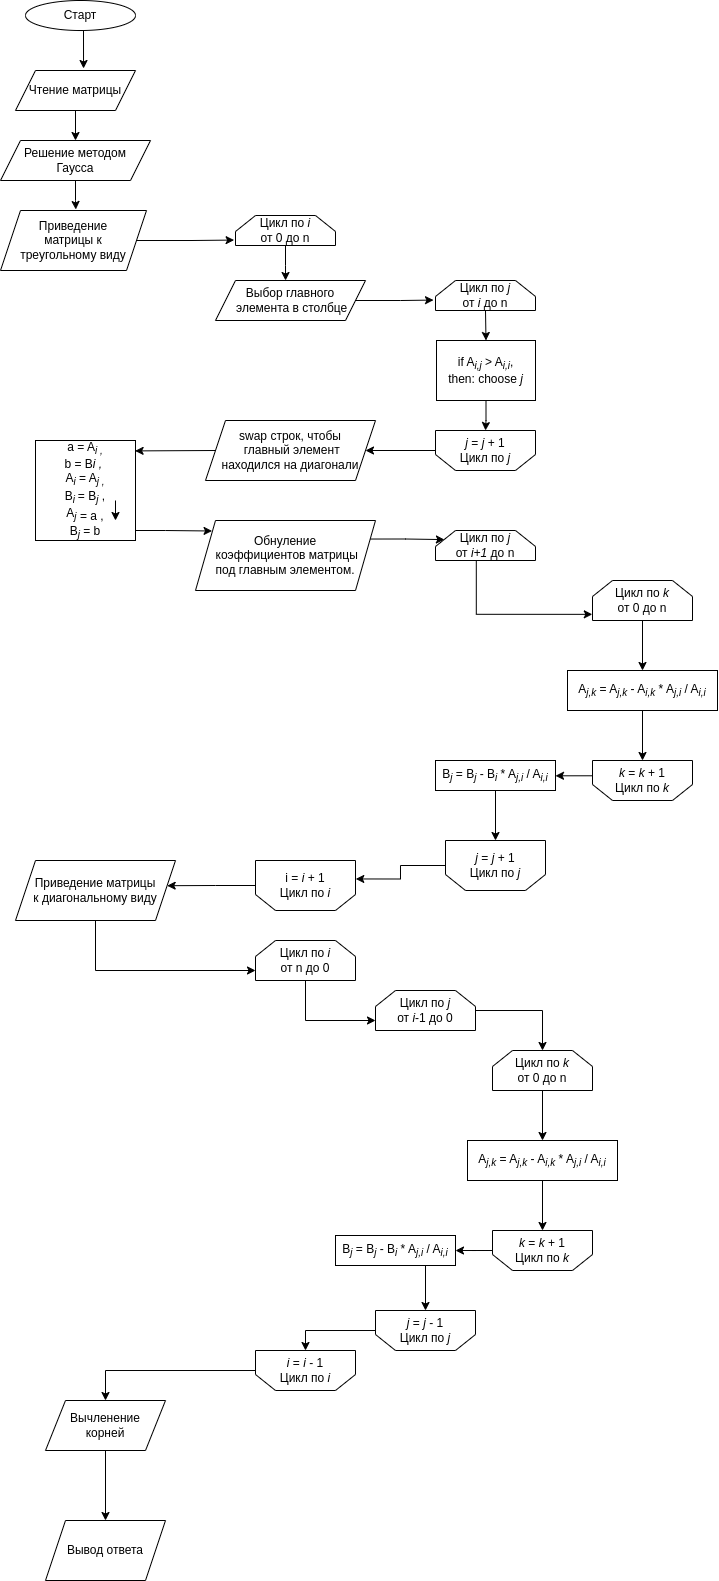
\includegraphics[scale=0.3]{img/блок-схема}
%\end{figure}

\subsubsection{Listing реализованного численного метода}
\tiny
\begin{verbatim}
    public class CalculateEquationWithChordMethodRealization implements CalculateEquationWithChordMethod {
    
    @Override
    public double calculate(SimpleFunction func, double a, double b, double x, double epsilon, long n) {
        if (n == 0) {
            x = a - (b - a) / (func.apply(b) - func.apply(a)) * func.apply(a);
            n++;
            if (func.apply(a) * func.apply(x) < 0) {
                return calculate(func, a, x, x, epsilon, n);
            } else if (func.apply(b) * func.apply(x) < 0) {
                return calculate(func, x, b, x, epsilon, n);
            } else {
                return x;
            }
        } else {
            double x_i = (a * func.apply(b) - b * func.apply(a)) / (func.apply(b) - func.apply(a));
            n++;
            if (Math.abs(x_i - x) > epsilon) {
                x = x_i;
                if (func.apply(a) * func.apply(x) < 0) {
                    return calculate(func, a, x, x, epsilon, n);
                } else if (func.apply(b) * func.apply(x) < 0) {
                    return calculate(func, x, b, x, epsilon, n);
                } else {
                    return x;
                }
            } else {
                return x_i;
            }
        }
    }
}
\end{verbatim}
\normalsize

\subsection{Метод простой итерации}

\subsubsection{Описание метода}


\subsubsection{Блок-схема численного метода}
d

\subsubsection{Listing реализованного численного метода}
\begin{verbatim}
    public class CalculateEquationWithSimpleIterationsMethodRealization implements CalculateEquationWithSimpleIterationsMethod {

    @Override
    public double[] chooseLyambdaAndX_0(SimpleFunction derivativeFunc, double a, double b) {
        double v1 = Math.abs(derivativeFunc.apply(a));
        double v2 = Math.abs(derivativeFunc.apply(b));
        double v = (-1) * (1 / Math.max(v1, v2));
        if (v1 > v2) return new double[]{v, a};
        else return new double[]{v, b};
    }

    @Override
    public double calculate(SimpleFunction func, double lyambda, double x, double epsilon) {
        double x_i = x + lyambda * func.apply(x);
        if (Math.abs(x_i - x) <= epsilon) {
            return x_i;
        } else {
            return calculate(func, lyambda, x_i, epsilon);
        }
    }
}

\end{verbatim}


\section{Решение систем нелинейных уравнений:}

\subsection{Метод Ньютона}

\subsubsection{Описание метода}
e

\subsubsection{Блок-схема численного метода}
f

\subsubsection{Listing реализованного численного метода}
\begin{verbatim}
    public class CalculateNSAEWithNewtonMethodRealization implements CalculateNSAEWithNewtonMethod {
    
    @Override
    public double[] calculate(double[] X, CreateMatrixForNewtoneMethod matrixCreator, double epsilon) throws MatrixCreateException, MatrixHasNoSolutionsException, TryCalculateNotDIagMatrixException {
        Matrix matrix = matrixCreator.create(X);
        MatrixCalulatorHandler calculator = new MatrixCalculatorHandlerImpl(matrix);
        calculator.transformToTriangleForm();
        double[] solutions = calculator.calcSolutions();
        double[] newX = new double[solutions.length];
        for (int i = 0; i < solutions.length; i++) {
            newX[i] = X[i] + solutions[i];
        }
        boolean flag = true;
        for (int i = 0; i < newX.length; i++) {
            if (Math.abs(newX[i] - X[i]) > epsilon) {
                flag = false;
                break;
            }
        }
        if (flag) {
            return newX;
        } else {
            return calculate(newX, matrixCreator, epsilon);
        }
    }
}

\end{verbatim}


\section{Examples}
\tiny
\begin{verbatim}
Enter "1" to solve the equation, enter "2" for NSAE:
\end{verbatim}\textbf{1}\begin{verbatim}
Choose the equation that you want to solve:
1. f(x) = sin(x)
2. f(x) = cos(x)
3. f(x) = x² - 1
4. f(x) = x³ - x + 4
5. f(n) = 2^n - 1
\end{verbatim}
\textbf{2}
\begin{verbatim}
The solution obtained by the chord method: 1.570783521943903
The solution obtained by the method of simple iterations: 4.712645995323825
\end{verbatim}

\begin{verbatim}
Enter "1" to solve the equation, enter "2" for NSAE:\end{verbatim} \textbf{2} \begin{verbatim}
Choose the NSAE that you want to solve:
1.  x² + y² - 4 = 0
    -3x² + y = 0

2.  cos(x) - y = 0
    sin(y) - x = 0
\end{verbatim}
\textbf{1}
\begin{verbatim}
Solutions: x1 = 0.7832125666191059
           x2 = 1.8402657654730223
\end{verbatim}
\normalsize

\section{Вывод}
g%Алгоритмическая сложность: O($N^3$)
%Отличие от простого Метода Гаусса - существенное уменьшение невязки, за счёт выбора главного элемента.
%Различие прямых методов от итерационных:
%\begin{enumerate}
%    \item Итерационным методом можно как быстрее найти решение, так и дольше - выше разброс, в то время, как прямой метод выполняется за определённое число итераций.
%    \item На больших матрицах у итерационных методов ниже погрешность и не накапливаются ошибки, в отличие от прямых.
%\end{enumerate}
%